

Intuitivamente, una función es \textbf{continua} si su gráfica se puede trazar sin levantar el lápiz del papel.\\
\\
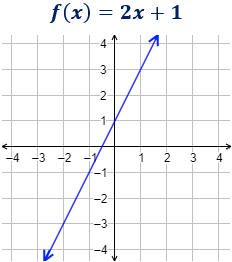
\includegraphics{samples/propiedades/funcionContinua.jpg}\\

Cuendo existen puntos en los que es necesario levantar el lápiz del papel, se dice que la función es \textbf{discontinua} en estos puntos, que se denominan \textbf{puntos de discontinuidad}.\\
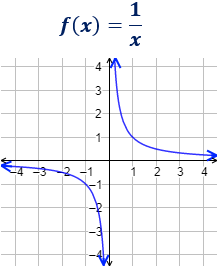
\includegraphics{samples/propiedades/funcionDiscontinua.jpg}

\subsubsection{Ejercicios}
\begin{ex}[sol later]
	Estudia la continuidad de las siguientes funciones::\\
	\begin{itemize}
		\item $f(x) = \dfrac{1}{x-2}$
		\item $f(x) = \dfrac{1}{3x^2-27}$
		\item $f(x) = \dfrac{x^2-2x}{2x^2+3x-2}$
		\item $f(x) = \sqrt{x^2+2x+1}$
		\item $f(x) = \sqrt{3x^2-3x-6}$
		\item $f(x) = \dfrac{\sqrt{x^2-1}}{x^4-x^3-x^2+x}$
		\item $f(x) = \dfrac{2x^2-x}{\sqrt{x^3+x^2-x-1}}$
		\item $f(x) = 3^{\dfrac{1}{x^2-1}}$
		\item $f(x) = \log(x^2-4x+4)$
	\end{itemize}
	\begin{sol}
		\begin{itemize}
			\item Dom(f) = $\mathbb{R}-\{2\}$. Función continua en todo su dominio.
			\item Dom(f) = $\mathbb{R}-\{-3,3\}$. Función continua en todo su dominio.
			\item Dom(f) = $\mathbb{R}-\{\dfrac{1}{2}\}$. Función continua en todo su dominio.
			\item Dom(f) = $\mathbb{R}$. Función continua en todo su dominio.
			\item Dom(f) = $(-\infty, -1] \bigcup [2,+\infty)$. Función continua en todo su dominio.
			\item Dom(f) = $\mathbb{R}-[-1,1]$. Función continua en todo su dominio.
			\item Dom(f) = $[1,+\infty)$. Función continua en todo su dominio.
			\item Dom(f) = $\mathbb{R}-\{-1, 1\}$. Función continua en todo su dominio.
			\item Dom(f) = $\mathbb{R}-\{2\}$. Función continua en todo su dominio.
		\end{itemize}
	\end{sol}
\end{ex}
